\documentclass[border=10pt]{standalone}
\usepackage{tikz}
\usetikzlibrary{arrows,positioning,shapes.geometric}

\begin{document}
    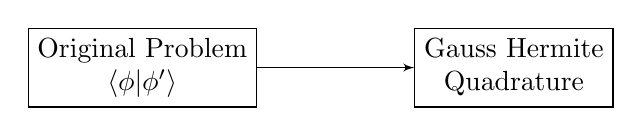
\begin{tikzpicture}[>=latex']
        \tikzset{block/.style= {draw, rectangle, align=center,minimum width=2cm,minimum height=1cm},
        rblock/.style={draw, shape=rectangle,rounded corners=1.5em,align=center,minimum width=2cm,minimum height=1cm},
        input/.style={
        draw,
        trapezium,
        trapezium left angle=60,
        trapezium right angle=120,
        minimum width=2cm,
        align=center,
        minimum height=1cm
        },
        }
        \node [block]  (op) {Original Problem \\ $\langle \phi | \phi^\prime \rangle$};
        \node [block, right =2cm of op] (gh) {Gauss Hermite \\ Quadrature};
        \path[draw,->] (op) -- (gh);
    \end{tikzpicture}
\end{document}
